\begin{figure}[t]
\centering
\resizebox{\textwidth}{!}{%
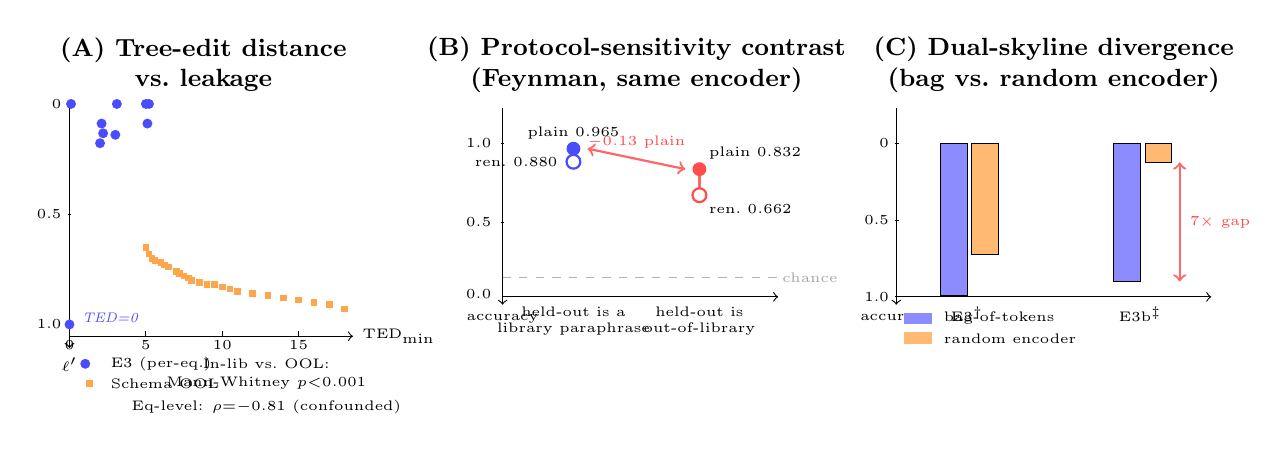
\begin{tikzpicture}[
  font=\small,
  lbl/.style={font=\footnotesize, align=center},
  hdrlbl/.style={font=\small\bfseries, align=center},
]

% ====================================================================
% PANEL A: TED scatter plot (structural distance vs leakage)
% ====================================================================
\node[hdrlbl] at (0, 0) {(A) Tree-edit distance\\vs.\ leakage};

% Y baseline
\def\AY{-0.5}

% Axes: x = TED (0 to 18), y = ell' (0 to 1.0)
% x scale: 18 TED units map to 3.5 cm
\def\Axscale{0.194}  % 3.5/18
% y scale: 1.0 ell' maps to 2.8 cm (downward)
\def\Ayscale{2.8}

\draw[->] (-1.7, \AY) -- (-1.7, \AY-\Ayscale-0.3)
  node[below, font=\tiny] {$\ell'$};
\draw[->] (-1.7, \AY-\Ayscale-0.15) -- (1.9, \AY-\Ayscale-0.15)
  node[right, font=\tiny] {TED$_{\min}$};

% Y ticks
\foreach \yv/\ylbl in {0.0/0, 0.5/0.5, 1.0/1.0} {
  \draw (-1.72, \AY-\yv*\Ayscale) -- (-1.68, \AY-\yv*\Ayscale)
    node[left, font=\tiny] {\ylbl};
}
% X ticks
\foreach \xv in {0, 5, 10, 15} {
  \draw (-1.7+\xv*\Axscale, \AY-\Ayscale-0.15) -- (-1.7+\xv*\Axscale, \AY-\Ayscale-0.08)
    node[below, font=\tiny] {\xv};
}

% E3 library points (blue circles): per-equation ℓ′ from r21 (n=25 seeds each)
% gaussian: TED=5, ℓ′=0.000; coulomb: TED=2, ℓ′=0.178; grav_pe: TED=2, ℓ′=0.089
% spring_pe: TED=5, ℓ′=0.089; capacitor_v: TED=3, ℓ′=0.140; wavenumber: TED=0, ℓ′=1.000
% cyclotron: TED=3, ℓ′=0.000; thermal: TED=2, ℓ′=0.133; energy_d: TED=5, ℓ′=0.000
% doppler: TED=0, ℓ′=0.000
\foreach \tx/\ty in {5/0.000, 2/0.178, 2.1/0.089, 5.1/0.089, 3/0.140, 0/1.000, 3.1/0.000, 2.2/0.133, 5.2/0.000, 0.1/0.000} {
  \fill[blue!70] (-1.7+\tx*\Axscale, \AY-\ty*\Ayscale) circle (1.8pt);
}
% wavenumber (TED=0, ℓ′≈1) annotated: trivially solvable (training duplicate)
\node[blue!70, font=\tiny, right] at (-1.7+0.2*\Axscale, \AY-0.97*\Ayscale) {\textit{TED=0}};

% r22 schema points (orange squares) — representative subset at varied TED/ell'
% TED~5: ell'~0.65-0.71; TED~7: ell'~0.75-0.80; TED~10: ell'~0.80-0.85; TED~14-18: ell'~0.88-0.93
\foreach \tx/\ty in {5/0.65, 5.2/0.68, 5.4/0.70, 5.6/0.71, 6/0.72, 6.2/0.73, 6.5/0.74, 7/0.76, 7.2/0.77, 7.5/0.78, 7.8/0.79, 8/0.80, 8.5/0.81, 9/0.82, 9.5/0.82, 10/0.83, 10.5/0.84, 11/0.85, 12/0.86, 13/0.87, 14/0.88, 15/0.89, 16/0.90, 17/0.91, 18/0.93} {
  \fill[orange!70] (-1.7+\tx*\Axscale, \AY-\ty*\Ayscale) +(-1.2pt,-1.2pt) rectangle +(1.2pt,1.2pt);
}

% Legend
\fill[blue!70] (-1.5, \AY-3.3) circle (1.8pt);
\node[right, font=\tiny] at (-1.3, \AY-3.3) {E3 (per-eq.)};
\fill[orange!70] (-1.45, \AY-3.55) +(-1.2pt,-1.2pt) rectangle +(1.2pt,1.2pt);
\node[right, font=\tiny] at (-1.3, \AY-3.55) {Schema OOL};

% Cluster contrast annotations
\node[font=\tiny, align=center] at (0.8, \AY-3.3) {In-lib vs.\ OOL:};
\node[font=\tiny, align=center] at (0.8, \AY-3.55) {Mann-Whitney $p{<}0.001$};
\node[font=\tiny, align=center] at (0.8, \AY-3.85) {Eq-level: $\rho{=}{-}0.81$ (confounded)};

% ====================================================================
% PANEL B: Generalization curve (E3 → E3m → E3b)
% ====================================================================
\def\Bx{5.5}

\node[hdrlbl] at (\Bx, 0) {(B) Protocol-sensitivity contrast\\(Feynman, same encoder)};

% Axes
\draw[->] (\Bx-1.7, \AY-0.05) -- (\Bx-1.7, \AY-2.55)
  node[below, font=\tiny] {accuracy};
\draw[->] (\Bx-1.7, \AY-2.45) -- (\Bx+1.8, \AY-2.45);

% Y axis labels (accuracy, 1.0 at top)
\node[left, font=\tiny] at (\Bx-1.72, \AY-0.50) {$1.0$};
\node[left, font=\tiny] at (\Bx-1.72, \AY-1.50) {$0.5$};
\node[left, font=\tiny] at (\Bx-1.72, \AY-2.42) {$0.0$};

% Y tick marks
\draw (\Bx-1.72, \AY-0.50) -- (\Bx-1.68, \AY-0.50);
\draw (\Bx-1.72, \AY-1.50) -- (\Bx-1.68, \AY-1.50);

% Two condition groups; each shows the (plain, renamed) PAIR -- the primary
% evidence. Numbers are Table 2 (matched 8-equation contrast, tag r33).
\def\xE{-0.8}
\def\xB{0.8}

% accuracy -> y: acc=1 at AY-0.50, acc=0 at AY-2.45  (y = -0.50 - (1-acc)*1.95)
\def\yEp{-0.568}   % in-library, plain    acc=0.965
\def\yEr{-0.734}   % in-library, renamed  acc=0.880
\def\yBp{-0.828}   % out-of-library, plain   acc=0.832
\def\yBr{-1.159}   % out-of-library, renamed acc=0.662
\def\yC{-2.206}    % chance (K=8)            acc=0.125

% chance line
\draw[gray!60, dashed] (\Bx-1.7, \AY+\yC) -- (\Bx+1.8, \AY+\yC)
  node[right, font=\tiny, gray!70, xshift=-2pt] {chance};

% within-condition drop under renaming
\draw[thick, blue!60] (\Bx+\xE, \AY+\yEp) -- (\Bx+\xE, \AY+\yEr);
\draw[thick, red!60]  (\Bx+\xB, \AY+\yBp) -- (\Bx+\xB, \AY+\yBr);

% in-library pair
\fill[blue!70] (\Bx+\xE, \AY+\yEp) circle (2.5pt);
\node[above, font=\tiny] at (\Bx+\xE, \AY+\yEp) {plain $0.965$};
\draw[blue!70, fill=white, thick] (\Bx+\xE, \AY+\yEr) circle (2.5pt);
\node[left, font=\tiny] at (\Bx+\xE-0.08, \AY+\yEr) {ren.\ $0.880$};

% out-of-library pair
\fill[red!70] (\Bx+\xB, \AY+\yBp) circle (2.5pt);
\node[above right, font=\tiny] at (\Bx+\xB, \AY+\yBp) {plain $0.832$};
\draw[red!70, fill=white, thick] (\Bx+\xB, \AY+\yBr) circle (2.5pt);
\node[below right, font=\tiny] at (\Bx+\xB, \AY+\yBr) {ren.\ $0.662$};

% the effect: plain accuracy itself collapses
\draw[<->, thick, red!60] (\Bx+\xE+0.18, \AY+\yEp) -- (\Bx+\xB-0.18, \AY+\yBp)
  node[midway, above, font=\tiny, red!70] {$-0.13$ plain};

% X axis labels (categorical protocol regimes)
\node[below, font=\tiny, align=center] at (\Bx+\xE, \AY-2.45) {held-out is a\\library paraphrase};
\node[below, font=\tiny, align=center] at (\Bx+\xB, \AY-2.45) {held-out is\\out-of-library};


% ====================================================================
% PANEL C: Dual-skyline divergence (grouped bar chart)
% ====================================================================
\def\Cx{10.8}

\node[hdrlbl] at (\Cx, 0) {(C) Dual-skyline divergence\\(bag vs.\ random encoder)};

% Axes
\draw[->] (\Cx-2.0, \AY-0.05) -- (\Cx-2.0, \AY-2.55)
  node[below, font=\tiny] {accuracy};
\draw[->] (\Cx-2.0, \AY-2.45) -- (\Cx+2.0, \AY-2.45);

% Y ticks
\foreach \yv/\ylbl in {0.0/0, 0.5/0.5, 1.0/1.0} {
  \draw (\Cx-2.02, \AY-0.5-\yv*1.95) -- (\Cx-1.97, \AY-0.5-\yv*1.95)
    node[left, font=\tiny] {\ylbl};
}

% Bar width
\def\bw{0.34}

% E3 group: centred at -1.1
% bag=0.992, random=0.724
\fill[blue!45] (\Cx-1.1-\bw, \AY-0.5) rectangle (\Cx-1.1, \AY-0.5-0.992*1.95);
\draw (\Cx-1.1-\bw, \AY-0.5) rectangle (\Cx-1.1, \AY-0.5-0.992*1.95);
\fill[orange!55] (\Cx-1.1+0.06, \AY-0.5) rectangle (\Cx-1.1+0.06+\bw, \AY-0.5-0.724*1.95);
\draw (\Cx-1.1+0.06, \AY-0.5) rectangle (\Cx-1.1+0.06+\bw, \AY-0.5-0.724*1.95);
\node[below, font=\tiny] at (\Cx-1.1, \AY-2.45) {E3$^{\dagger}$};

% E3b group: centred at +1.1
% bag=0.900, random=0.124
\fill[blue!45] (\Cx+1.1-\bw, \AY-0.5) rectangle (\Cx+1.1, \AY-0.5-0.900*1.95);
\draw (\Cx+1.1-\bw, \AY-0.5) rectangle (\Cx+1.1, \AY-0.5-0.900*1.95);
\fill[orange!55] (\Cx+1.1+0.06, \AY-0.5) rectangle (\Cx+1.1+0.06+\bw, \AY-0.5-0.124*1.95);
\draw (\Cx+1.1+0.06, \AY-0.5) rectangle (\Cx+1.1+0.06+\bw, \AY-0.5-0.124*1.95);
\node[below, font=\tiny] at (\Cx+1.1, \AY-2.45) {E3b$^{\ddagger}$};

% Divergence annotation
\draw[<->, thick, red!60] (\Cx+1.1+0.06+\bw+0.1, \AY-0.5-0.900*1.95) --
  (\Cx+1.1+0.06+\bw+0.1, \AY-0.5-0.124*1.95)
  node[midway, right, font=\tiny, red!70, align=left] {$7{\times}$ gap};

% Legend
\fill[blue!45] (\Cx-1.9, \AY-2.65) rectangle (\Cx-1.55, \AY-2.80);
\node[right, font=\tiny] at (\Cx-1.52, \AY-2.725) {bag-of-tokens};
\fill[orange!55] (\Cx-1.9, \AY-2.90) rectangle (\Cx-1.55, \AY-3.05);
\node[right, font=\tiny] at (\Cx-1.52, \AY-2.975) {random encoder};

\end{tikzpicture}%
}
\caption{Three complementary views of variable-identity leakage. \textbf{(A)}~Tree-edit-distance scatter: in-library forms show per-equation $\ell'$ ($n{=}25$ seeds each), schema-generated out-of-library forms show per-form $\ell'$. One in-library equation (wavenumber, TED$=0$) sits at $\ell'{\approx}1$ because its held-out form is a training duplicate; it and the other TED$=0$ form are excluded from the headline contrast. The two TED distributions are separated (Mann--Whitney $p{<}0.001$) but \emph{overlap}; the equation-level correlation is $\rho{=}{-}0.81$ ($p{=}0.004$) while the residualized within-equation correlation is $\rho{=}{+}0.52$ ($p{<}0.001$): a Simpson's-paradox reversal we interpret in \S\ref{sec:coverage} without leaning on either sign. \textbf{(B)}~The matched contrast of Table~\ref{tab:diversity_sweep}, reported as \emph{(plain, renamed) pairs} rather than as an index: on one equation set of eight, one encoder and one training procedure, changing only how the held-out form is constructed drops plain accuracy by $0.13$ and renamed accuracy by $0.22$. \textbf{(C)}~Dual-skyline divergence as a distribution-shift diagnostic: in-distribution, bag and random encoder track each other; under out-of-library shift they diverge $7\times$ on identical forms with an identical centroid protocol.}
\label{fig:overview}
\end{figure}
